\documentclass[border=0.2cm]{standalone}
\usepackage{pgfplots}
\pgfplotsset{compat=1.18}

% Define custom colors
\definecolor{testcolor}{RGB}{250, 164, 58}  % Orange for test

\begin{document}

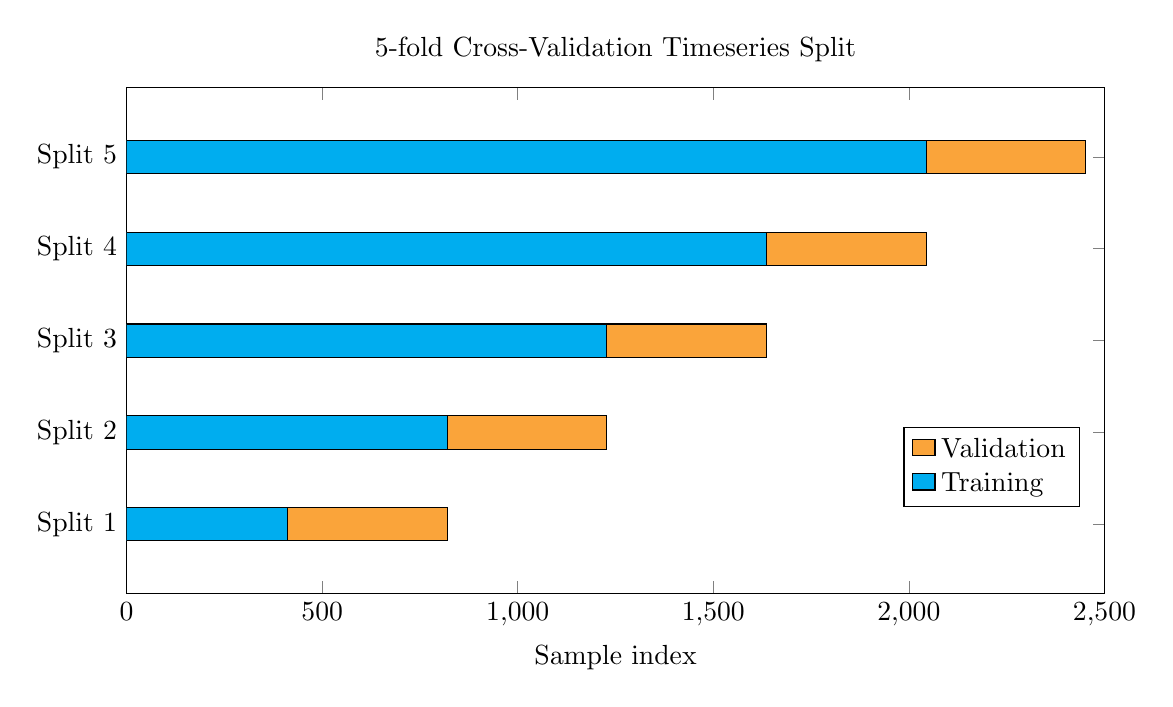
\begin{tikzpicture}

\begin{axis}[
    xbar stacked, % Stacked bar style
    bar width=12pt,
    xmin=0, 
    xmax=2500, 
    xlabel={Sample index},
    ytick={0,1,2,3,4},
    title={5-fold Cross-Validation Timeseries Split},
    yticklabels={Split 1, Split 2, Split 3, Split 4, Split 5},
    xtick={0,500,1000,1500,2000,2500}, % Set x ticks at intervals of 500
    enlarge y limits={abs=0.75},
    legend style={at={(0.975,0.25)}, anchor=east, legend columns=1}, % Move legend to the right
    legend cell align={left},
    reverse legend, % Match the order of entries in the legend
    width=14cm,
    height=8cm,
]

% Orange bars (Train)
\addplot[fill=cyan] coordinates {(412,0) (820,1) (1228,2) (1636,3) (2044,4)};

% Blue bars (Test)
\addplot[fill=testcolor] coordinates {(408,0) (408,1) (408,2) (408,3) (408,4)};

\legend{Training, Validation}

\end{axis}

\end{tikzpicture}

\end{document}
